\documentclass[prl,aps,twocolumn,floatfix,amsmath,amssymb,superscriptaddress,tightenlines]{revtex4}
\usepackage{graphicx}
%\usepackage{epstopdf}
\usepackage{amsfonts}
\usepackage{bm}
\usepackage{color}
\begin{document}

\date{\today}
\title{Measuring Renyi Entanglement Entropy with Quantum Monte Carlo}

%\author{Ann B. Kallin}
%\affiliation{Department of Physics and Astronomy, University of Waterloo, Ontario, N2L 3G1, Canada} 
%
%\author{Iv\'an Gonz\'alez}
%\affiliation{Centro de Supercomputaci\'on de Galicia, Avda.~de~Vigo~s/n, E-15705 Santiago de Compostela, Spain}
%
%\author{Matthew B. Hastings}
%\affiliation{Microsoft Research, Station Q, CNSI Building, University of California, Santa Barbara, CA, 93106}
%
%\author{Roger G. Melko}
%\affiliation{Department of Physics and Astronomy, University of Waterloo, Ontario, N2L 3G1, Canada} 

\begin{abstract} 
We develop a procedure for measuring the entanglemenet entropy of a region $A$ in a quantum
many-body system using valence-bond basis quantum Monte Carlo simulations.  Specifically, an 
estimator for the so-called Renyi $\alpha$-entropy, with $\alpha = 2$, is related to the expectation of
a unitary operator which swaps the basis states of a region $A$ with an ancillary copy of that region.
We demonstrate that the Renyi entropy calculated for a Heisenberg model in quantum Monte Carlo 
converges to exact results provided by density matrix renormalization group calculations.  Finally, we 
calculate the scaling of the Renyi entropy in the 2D Heisenberg model and confirm that the N\'eel 
groundstate obeys the expected area law.
\end{abstract}
\maketitle

{\it Introduction.}-- 
The measurement of entanglement in interacting quantum many-body systems has promised to provide
new tools and insight to the field of condensed-matter physics.  Most exciting are proposals to use 
entanglement as a probe to detect topological order, for example in paramagnetic spin liquids with no 
local order parameters, and fractional quantum hall states important in proposals for topologically protected qbits.  
A variety of measures of entanglement entropy are used, including fidelity, concurrence, and entropy, the 
latter being perhaps the most widely studied.  The general belief is that in two dimensions (2D) and higher, the 
leading contribution to the entanglement entropy scales as the boundary of a subsystem $A$ -- the so-called
``area law''.  In additional to important corrections in topological phases, subleading universal corrections are
believed to occur in the presence of a quantum critical point, or because of the presence of ``corners'' in the region
$A$.  Thus, the study of entanglement entropy would provide a rich new avenue for the study of ...

A major obstacle in the use of entanglement entropy as a resource for studying condensed-matter systems is 
the difficulty in calculating it numerically in 2D and higher.

Consider the Renyi entropy, defined as 
\begin{equation}
S_{\alpha} (\rho_A) = \frac{1}{1- \alpha} \ln \left[{ {\rm Tr}\big( \rho_A^{\alpha} \big) }\right],
\end{equation}
where $\rho_A$ is the reduced-density matrix of a subregion $A$ entangled with its complement $B$, and 
$\alpha$ is a positive-definite integer parameter.  In the limit $\alpha \rightarrow 1$, one recovers the formal 
definition of the von Neumann entropy, $S_1 (\rho_A) = - {\rm Tr}( \rho_A \ln \rho_A )$.  The von Neumann entropy
is accessible numerically only in procedures where the reduced density matrix can be calculated directly, such as Lanczos 
or DMRG.  Scalable simulations methods in $D>1$, needed in order to study the groundstate, finite-temperature, and 
critical properties of the vast majority of systems of interested to condensed-matter physics, are so far essentially
restricted to quantum Monte Carlo (QMC).  In QMC, the wavefunction if the system is sampled inside of the trace...

 von Neumann entropy is 

\begin{figure} {
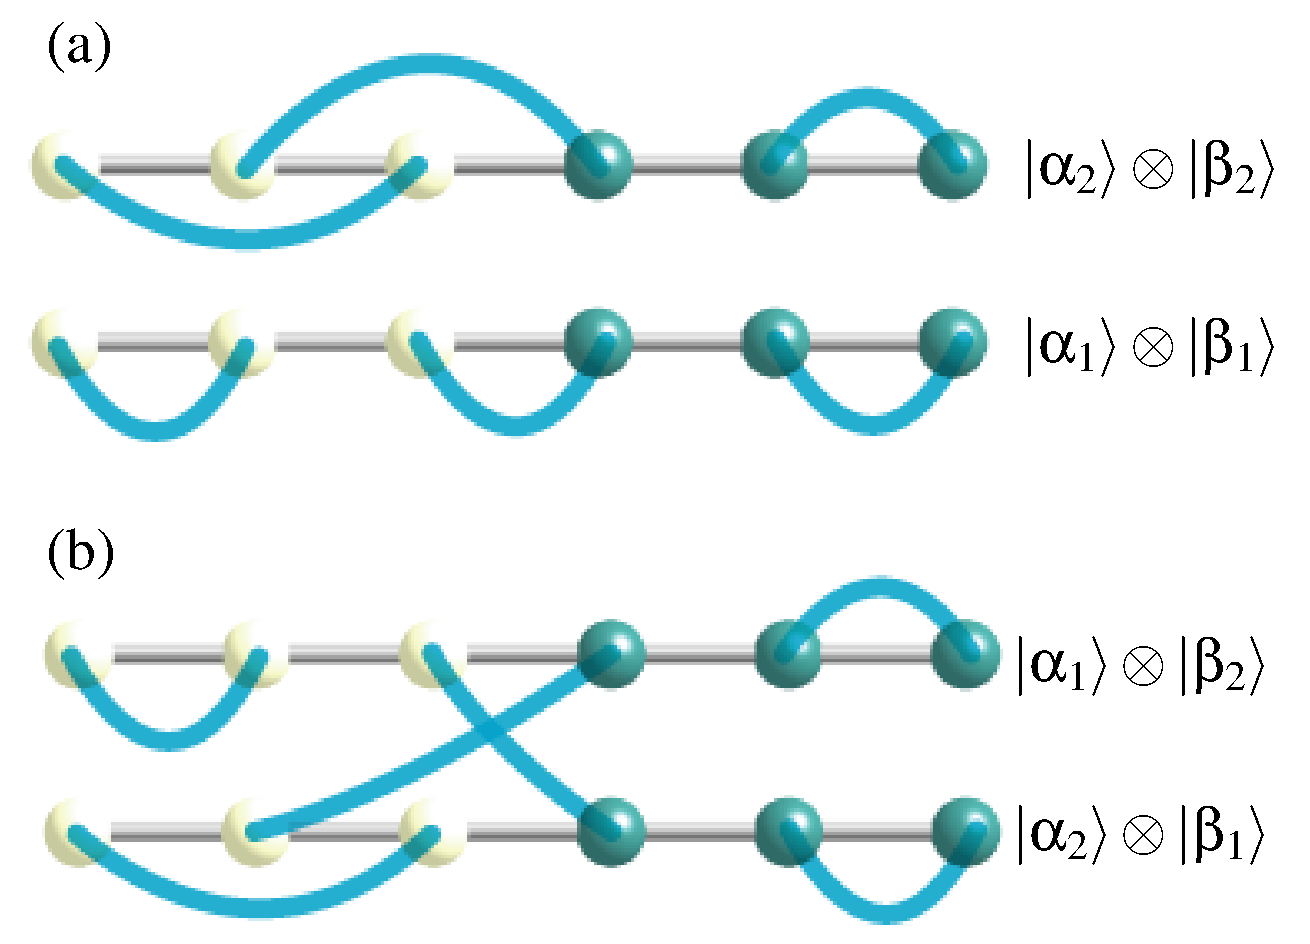
\includegraphics[width=2in]{swap_2.eps} \caption{(color online) 
\label{swap_2}}} \end{figure}


{\it Acknowledgments.}-- The authors thank ...
This work was made possible by the
computing facilities of SHARCNET and CESGA.  Support was provided by NSERC
of Canada (A.B.K. and R.G.M.) and the NSF under Grant No. NSF PHY05-51164
(I.G.).

\bibliography{Biblio}

\end{document}
